\documentclass[11pt]{exam}
\usepackage[margin=1in]{geometry}
\usepackage{amsfonts, amsmath, amssymb, amsthm}
\usepackage{mathtools}
\usepackage{enumerate}
\usepackage{listings}
\usepackage{colortbl}
\usepackage{float}
\usepackage{tikz}
\usepackage[colorlinks,linkcolor=blue]{hyperref}

% in order to compile this file you need to get 'header.tex' from
% Canvas and change the line below to the appropriate file path
%%% theorems

\theoremstyle{plain}            % following are "theorem" style
\newtheorem{theorem}{Theorem}[section]
\newtheorem{lemma}[theorem]{Lemma}
\newtheorem{corollary}[theorem]{Corollary}
\newtheorem{proposition}[theorem]{Proposition}
\newtheorem{claim}[theorem]{Claim}
\newtheorem{fact}[theorem]{Fact}
\newtheorem{openproblem}[theorem]{Open Problem}

\theoremstyle{definition}       % following are def style
\newtheorem{definition}[theorem]{Definition}
\newtheorem{conjecture}[theorem]{Conjecture}
\newtheorem{example}[theorem]{Example}
\newtheorem{protocol}[theorem]{Protocol}
\newtheorem{exercise}[theorem]{Exercise}

\theoremstyle{remark}           % following are remark style
\newtheorem{remark}[theorem]{Remark}
\newtheorem{note}[theorem]{Note}
%\newtheorem*{solution}{Solution}

%%% special sets
\newcommand{\bit}{\ensuremath{\{0,1\}}}
\newcommand{\bitt}{\ensuremath{\{-1,1\}}}
\newcommand{\ball}{\ensuremath{\mathcal{B}}}
\newcommand{\sph}{\ensuremath{\mathbb{S}}}
\newcommand{\odisc}[2]{\ensuremath{D(#1, #2)}}
\newcommand{\cdisc}[2]{\ensuremath{\bar{D}(#1, #2)}}
\newcommand{\emp}{\varnothing}

% constants
\newcommand{\E}{\ensuremath{\mathrm{e}}}
\newcommand{\I}{\ensuremath{\mathrm{i}}}
\newcommand{\Id}{\ensuremath{\mathrm{I}}}
\newcommand{\paulix}{\ensuremath{\mathrm{X}}}
\newcommand{\pauliy}{\ensuremath{\mathrm{Y}}}
\newcommand{\pauliz}{\ensuremath{\mathrm{Z}}}

% font for general-purpose algorithms
\newcommand{\algo}[1]{\ensuremath{\mathsf{#1}}}
% font for general-purpose computational problems
\newcommand{\problem}[1]{\ensuremath{\mathsf{#1}}}
% font for complexity classes
\newcommand{\class}[1]{\ensuremath{\mathsf{#1}}}

% asymptotics
\DeclareMathOperator{\poly}{poly}
\DeclareMathOperator{\polylog}{polylog}
\DeclareMathOperator{\negl}{negl}
\DeclareMathOperator{\bigO}{O}
\DeclareMathOperator{\litO}{o}
\DeclareMathOperator{\Otil}{\tilde{O}}
\DeclareMathOperator{\Ostar}{O^*}

%%% "LEFT-RIGHT" PAIRS OF SYMBOLS

% inner product
\DeclarePairedDelimiter\inner{\langle}{\rangle}
% absolute value
\DeclarePairedDelimiter\abs{\lvert}{\rvert}
% a set
\DeclarePairedDelimiter\set{\{}{\}}
% parens
\DeclarePairedDelimiter\parens{(}{)}
% tuple, alias for parens
\DeclarePairedDelimiter\tuple{(}{)}
% square brackets
\DeclarePairedDelimiter\bracks{[}{]}
% rounding off
\DeclarePairedDelimiter\round{\lfloor}{\rceil}
% floor function
\DeclarePairedDelimiter\floor{\lfloor}{\rfloor}
% ceiling function
\DeclarePairedDelimiter\ceil{\lceil}{\rceil}
% length of some vector, element
\DeclarePairedDelimiter\length{\lVert}{\rVert}
% "lifting" of a residue class
\DeclarePairedDelimiter\lift{\llbracket}{\rrbracket}
\DeclarePairedDelimiter\len{\lvert}{\rvert}
% bra-kets
\DeclarePairedDelimiter\bra{\langle}{\rvert}
\DeclarePairedDelimiter\ket{\lvert}{\rangle}
\newcommand{\braket}[2]{\ensuremath{\langle #1 \vert #2 \rangle}}
\newcommand{\ketbra}[2]{\ensuremath{\lvert #1 \rangle \langle #2 \rvert}}

%%% spacing

\newcommand{\ws}{\hspace{1pt}}
\newcommand{\wws}{\hspace{2pt}}
\newcommand{\hs}{\hspace{4pt}}
\newcommand{\hhs}{\hspace{8pt}}
\newcommand{\hhhs}{\hspace{12pt}}

%%% LISTS

\newcommand{\oneto}{1, \ldots,}
\newcommand{\onetop}{1 \cdots,}
\newcommand{\zeroto}{0, \ldots,}
\newcommand{\zerotop}{0 \cdots,}
\newcommand{\perm}[1]{\mathbf{(#1)}}
\newcommand{\permv}[1]{(#1)}
\newcommand{\varind}[2]{#1_1, \ldots, #1_#2}
\newcommand{\varindz}[2]{#1_0, \ldots, #1_#2}
\newcommand{\varindp}[2]{#1_1 \cdots #1_#2}
\newcommand{\varindpz}[2]{#1_0 \cdots #1_#2}
\newcommand{\seq}[2]{(#1_#2)_{#2=1}^\infty}
\newcommand{\seqz}[2]{(#1_#2)_{#2=0}^\infty}

%%% MATH OPERATORS

%\DeclareMathOperator{\pr}{\mathbf{P}}
%\DeclareMathOperator{\ex}{\mathbf{E}}
\DeclareMathOperator{\pr}{P}
\DeclareMathOperator{\ex}{E}
\DeclareMathOperator{\Span}{Span}
\DeclareMathOperator{\tr}{Tr}
\DeclareMathOperator{\supp}{Supp}
\DeclareMathOperator{\im}{Im}
\DeclareMathOperator{\var}{var}
\DeclareMathOperator{\vol}{vol}
\DeclareMathOperator{\sign}{sign}
\DeclareMathOperator{\dkl}{D_{KL}}
\DeclareMathOperator{\entr}{H}
\DeclareMathOperator{\fid}{F}
\DeclareMathOperator{\dist}{D}
\DeclareMathOperator{\ad}{ad}

% hats

\newcommand{\fhat}{\ensuremath{\hat{f}}}
\newcommand{\phat}{\ensuremath{\hat{p}}}
\newcommand{\that}{\ensuremath{\hat{t}}}

%%% BLACKBOARD SYMBOLS

% \newcommand{\C}{\ensuremath{\mathbb{C}}}
\newcommand{\D}{\ensuremath{\mathbb{D}}}
\newcommand{\F}{\ensuremath{\mathbb{F}}}
% \newcommand{\G}{\ensuremath{\mathbb{G}}}
\newcommand{\J}{\ensuremath{\mathbb{J}}}
\newcommand{\N}{\ensuremath{\mathbb{N}}}
\newcommand{\Q}{\ensuremath{\mathbb{Q}}}
\newcommand{\R}{\ensuremath{\mathbb{R}}}
\newcommand{\T}{\ensuremath{\mathbb{T}}}
\newcommand{\Z}{\ensuremath{\mathbb{Z}}}
\newcommand{\QR}{\ensuremath{\mathbb{QR}}}

% sets in calligraphic type

\newcommand{\calD}{\ensuremath{\mathcal{D}}}
\newcommand{\calF}{\ensuremath{\mathcal{F}}}
\newcommand{\calG}{\ensuremath{\mathcal{G}}}
\newcommand{\calH}{\ensuremath{\mathcal{H}}}
\newcommand{\calI}{\ensuremath{\mathcal{I}}}
\newcommand{\calL}{\ensuremath{\mathcal{L}}}
\newcommand{\calN}{\ensuremath{\mathcal{N}}}
\newcommand{\calP}{\ensuremath{\mathcal{P}}}
\newcommand{\calS}{\ensuremath{\mathcal{S}}}
\newcommand{\calX}{\ensuremath{\mathcal{X}}}
\newcommand{\calY}{\ensuremath{\mathcal{Y}}}

% matrices and vectors

\newcommand{\matA}{\ensuremath{\mathbf{A}}}
\newcommand{\matB}{\ensuremath{\mathbf{B}}}
\newcommand{\matC}{\ensuremath{\mathbf{C}}}
\newcommand{\matD}{\ensuremath{\mathbf{D}}}
\newcommand{\matE}{\ensuremath{\mathbf{E}}}
\newcommand{\matF}{\ensuremath{\mathbf{F}}}
\newcommand{\matG}{\ensuremath{\mathbf{G}}}
\newcommand{\matH}{\ensuremath{\mathbf{H}}}
\newcommand{\matI}{\ensuremath{\mathbf{I}}}
\newcommand{\matJ}{\ensuremath{\mathbf{J}}}
\newcommand{\matK}{\ensuremath{\mathbf{K}}}
\newcommand{\matL}{\ensuremath{\mathbf{L}}}
\newcommand{\matM}{\ensuremath{\mathbf{M}}}
\newcommand{\matN}{\ensuremath{\mathbf{N}}}
\newcommand{\matO}{\ensuremath{\mathbf{O}}}
\newcommand{\matP}{\ensuremath{\mathbf{P}}}
\newcommand{\matQ}{\ensuremath{\mathbf{Q}}}
\newcommand{\matR}{\ensuremath{\mathbf{R}}}
\newcommand{\matS}{\ensuremath{\mathbf{S}}}
\newcommand{\matT}{\ensuremath{\mathbf{T}}}
\newcommand{\matU}{\ensuremath{\mathbf{U}}}
\newcommand{\matV}{\ensuremath{\mathbf{V}}}
\newcommand{\matW}{\ensuremath{\mathbf{W}}}
\newcommand{\matX}{\ensuremath{\mathbf{X}}}
\newcommand{\matY}{\ensuremath{\mathbf{Y}}}
\newcommand{\matZ}{\ensuremath{\mathbf{Z}}}
\newcommand{\matzero}{\ensuremath{\mathbf{0}}}

\newcommand{\veca}{\ensuremath{\mathbf{a}}}
\newcommand{\vecb}{\ensuremath{\mathbf{b}}}
\newcommand{\vecc}{\ensuremath{\mathbf{c}}}
\newcommand{\vecd}{\ensuremath{\mathbf{d}}}
\newcommand{\vece}{\ensuremath{\mathbf{e}}}
\newcommand{\vecf}{\ensuremath{\mathbf{f}}}
\newcommand{\vecg}{\ensuremath{\mathbf{g}}}
\newcommand{\vech}{\ensuremath{\mathbf{h}}}
\newcommand{\veck}{\ensuremath{\mathbf{k}}}
\newcommand{\vecm}{\ensuremath{\mathbf{m}}}
\newcommand{\vecp}{\ensuremath{\mathbf{p}}}
\newcommand{\vecq}{\ensuremath{\mathbf{q}}}
\newcommand{\vecr}{\ensuremath{\mathbf{r}}}
\newcommand{\vecs}{\ensuremath{\mathbf{s}}}
\newcommand{\vect}{\ensuremath{\mathbf{t}}}
\newcommand{\vecu}{\ensuremath{\mathbf{u}}}
\newcommand{\vecv}{\ensuremath{\mathbf{v}}}
\newcommand{\vecw}{\ensuremath{\mathbf{w}}}
\newcommand{\vecx}{\ensuremath{\mathbf{x}}}
\newcommand{\vecy}{\ensuremath{\mathbf{y}}}
\newcommand{\vecz}{\ensuremath{\mathbf{z}}}
\newcommand{\veczero}{\ensuremath{\mathbf{0}}}
\newcommand{\vecone}{\ensuremath{\mathbf{1}}}

\newcommand{\vecell}{\ensuremath{\boldsymbol\ell}}
\newcommand{\vecalpha}{\ensuremath{\boldsymbol\alpha}}
\newcommand{\vecbeta}{\ensuremath{\boldsymbol\beta}}
\newcommand{\veceta}{\ensuremath{\boldsymbol\eta}}
\newcommand{\vecmu}{\ensuremath{\boldsymbol\mu}}
\newcommand{\vecphi}{\ensuremath{\boldsymbol\phi}}
\newcommand{\vecsigma}{\ensuremath{\boldsymbol\sigma}}
\newcommand{\vectheta}{\ensuremath{\boldsymbol\theta}}
\newcommand{\vecxi}{\ensuremath{\boldsymbol\xi}}

%%% misc

\newcommand{\ind}{\ensuremath{\mathbf{1}}}

\newcommand{\congmod}[3]{#1 \equiv #2 \textrm{ modulo } #3}

\newcommand{\dee}{\,\mathrm{d}}
\newcommand{\de}{\mathrm{d}}
\newcommand{\dx}{\,\mathrm{d} x}

\newcommand{\ol}{\overline}
\newcommand{\inv}[1]{\ensuremath{#1^{-1}}}
\newcommand{\tsp}[1]{\ensuremath{#1^{\top}}}


\newcommand{\eps}{\varepsilon}
\newcommand{\ph}{\varphi}

\newcommand{\Ra}{\Rightarrow}
\newcommand{\Lra}{\Leftrightarrow}
\newcommand{\rsqa}{\rightsquigarrow}

\newcommand{\trl}{\triangleleft}
\newcommand{\trr}{\triangleright}

\newcommand{\func}[3]{#1: #2 \to #3}
\newcommand{\dd}[1]{\frac{\mathrm{d}}{\mathrm{d}#1}}
\newcommand{\ptl}[1]{\frac{\partial}{\partial #1}}
\newcommand{\prtl}[2]{\frac{\partial #1}{\partial #2}}

\newcommand{\matrixtt}[4]{
  \begin{pmatrix*}[r]
        #1 & #2 \\
        #3 & #4
    \end{pmatrix*}
}

%%% for homework and section notes

\newcommand{\commonheader}[2]{
    \pagestyle{headandfoot}
    \setlength{\headheight}{26pt}
    \setlength{\headsep}{30pt}

    \header
        {\small{\textbf{VE281: Data Structures and Algorithms}} \\ \footnotesize{\textbf{UM-SJTU Joint Institute, SU2022}}}
        {#1}
        {#2}

    \firstpageheadrule
    \runningheadrule

    \footer
        {}
        {\thepage}
        {}
}

\newcommand{\hwheader}{
    \commonheader
        {\textbf{Homework \hwnum}}
        {\small \textbf{Due at \duedate}}
}

\newcommand{\hwslnheader}{
    \commonheader
    	{}
        {\textbf{Solutions to Homework \hwnum}}
    \printanswers
}

\newcommand{\notesheader}{
    \commonheader
        {\Large \textbf{Section Notes \sectionnum}}
    	{}
}

\newcommand{\hint}[1]{
\emph{Hint}: #1
}

% for effort questions
\let\Eitem=\relax
\def\effortE{\textbf{E}~}
\makeatletter
\def\Eitem{%
    \expandafter\let\expandafter\originallabel\csname labelenum\romannumeral\@enumdepth\endcsname
    \expandafter\def\csname labelenum\romannumeral\@enumdepth\expandafter\endcsname\expandafter{%
        \expandafter\effortE\originallabel}%
    \item
    \expandafter\let\csname labelenum\romannumeral\@enumdepth\endcsname\originallabel
}
\makeatother

\allowdisplaybreaks


\geometry{left=2.5 cm,right=2.5 cm,top=2.5 cm,bottom=2.5 cm}
%\pagestyle{fancy}
\definecolor{mygreen}{rgb}{0,0.6,0}  
\definecolor{mygray}{rgb}{0.5,0.5,0.5}
\definecolor{mymauve}{rgb}{0.58,0,0.82} 
\definecolor{background}{rgb}{0.963,0.963,0.963}

\definecolor{codegreen}{rgb}{0,0.6,0}
\definecolor{codegray}{rgb}{0.5,0.5,0.5}
\definecolor{codepurple}{rgb}{0.58,0,0.82}
\definecolor{backcolour}{rgb}{0.95,0.95,0.92}

\lstdefinestyle{mystyle}{
    backgroundcolor=\color{backcolour},   
    commentstyle=\color{codegreen},
    keywordstyle=\color{magenta},
    numberstyle=\tiny\color{codegray},
    stringstyle=\color{codepurple},
    basicstyle=\ttfamily\footnotesize,
    breakatwhitespace=false,         
    breaklines=true,                 
    captionpos=b,                    
    keepspaces=true,                 
    numbers=left,                    
    numbersep=5pt,                  
    showspaces=false,                
    showstringspaces=false,
    showtabs=false,                  
    tabsize=2
}

\lstset{style=mystyle}
\newcommand{\hwnum}{3}
\newcommand{\duedate}{11:59pm, July 8th}

%\notesheader
\hwheader   % header for homework
%\hwslnheader   % header for homework solutions

% Comment the following line in order to hide solutions.
% Uncomment the line to show solutions written inside of
% LaTeX solution environments like:
%   \begin{solution}
%     My solution.
%   \end{solution}.
\printanswers

\begin{document}
\setlength{\parindent}{0pt}
\section*{Before you start:}

\subsection*{Homework Files}
You can download the starter files for coding as well as this \textit{tex} file (you only need to modify \textit{homework3.tex}) on canvas and do your homework with latex. Or you can scan your handwriting, convert to pdf file, and upload it to canvas before the due date. If you choose to write down your answers by hand, you can directly download the pdf file on canvas which provides more blank space for solution box.\\

\subsection*{Submission Form}
A pdf file as your solution named as VE281\_HW3\_[Your Student ID]\_[Your name].pdf uploaded to canvas


Estimated time used for this homework: \textbf{3-4 hours.}
\\\\


\newpage
\section*{0\quad Student Info}
Your name and student id: Yinchen Ni ~ 520370910026
\begin{solution}
% Write your answer here
\end{solution}

\section{Tree Traversal (26 points)}

\subsection{Given A Tree (16 points)}
Given a binary tree below, please write out the following traversals:
\begin{figure}[H]
\centering
\includegraphics[width=.5\linewidth]{binary_tree.png}
\end{figure}
\begin{enumerate}[(a)]
\item Pre-order depth-first traversal. (4 points)
\begin{solution}
ABDHEIMJCFGKNL
\end{solution}

\item Post-order depth-first traversal. (4 points)
\begin{solution}
HDMIJEBFNKLGCA
\end{solution}

\item In-order depth-first traversal. (4 points)
\begin{solution}
HDBIMEJAFCNJGL
\end{solution}

\item Level-order traversal. (4 points)
\begin{solution}
ABCDEFGHIJKLMN
\end{solution}

\end{enumerate}


\subsection{Draw The Tree (10 points)}
\begin{enumerate}[a)]
\item Now we have a specific binary tree, but we only know some of its traversals. Its pre-order traversal is: \textbf{GCABFEDIHKJ}, and its in-order traversal is: \textbf{ABCDEFGHIJK}. Then please \textbf{draw out the binary tree} and show its \textbf{post-order traversal}. (4 points)

\begin{solution}
    \par 
    \begin{center}
    \begin{tikzpicture}[scale=0.8]
        \tikzstyle{every node}=[draw,shape=circle, minimum size=0.8cm];
        \node {G}[sibling distance=6cm]
        child { node {C}[sibling distance=3cm]
            child {
                node {A}[sibling distance=1.5cm]
                child [ missing ]
                child { node {B} }
            }
            child {
                node {F}[sibling distance=1.5cm]
                child { node {E}[sibling distance = 0.75cm]
                    child { node {D} }
                    child [missing]
                }
                child [ missing ]
            }
        }
        child { node {I}[sibling distance=3cm]
            child { node {H}}
            child {
                node {K}[sibling distance=1.5cm]
                child { node {J} }
                child [ missing ]
            }
        };
    \end{tikzpicture}
    \end{center}
\end{solution}

\item Now we have a specific binary tree, but we only know some of its traversals. Its post-order traversal is: \textbf{BDCAGIKJHFE}, and its in-order traversal is: \textbf{ABCDEFGHIJK}. Then please \textbf{draw out the binary tree} and show its \textbf{pre-order traversal}. (4 points)

\begin{solution}
    \par 
    \begin{center}
    \begin{tikzpicture}[scale=0.8]
        \tikzstyle{every node}=[draw,shape=circle, minimum size=0.8cm];
        \node {E}[sibling distance=6cm]
        child { node {A}[sibling distance=3cm]
            child [missing]
            child {
                node {C}[sibling distance=1.5cm]
                child { node {B}}
                child { node {D}}
            }
        }
        child { node {F}[sibling distance=3cm]
            child [missing]
            child { node {H}[sibling distance=1.5cm]
                child { node {G}}
                child { node {J}[sibling distance=1.5cm]
                    child {node {I}}
                    child {node {K}}
                }
            }
        };
    \end{tikzpicture}
    \end{center}
\end{solution}

\item After finishing the previous two questions, our smart Mr. Blue Tiger decides to publish paper title \textbf {New discovery!! Any pair of 2 distinctive DFS sequences has one and only one corresponding binary tree.} (distinctive here means following different order of DFS)
However, our strong TAA Chengyu does not seem to agree with Mr. Blue Tiger. He decides to publish another paper to explain why Mr. Blue Tiger's statement is wrong. Could you briefly explain the reasons? A more detailed statement should be made. (Hint: This problem is related to different combinations of distinctive DFS sequences, i.e. which two out of three orders are picked as known sequences)

\begin{solution}
The pre-order traversal combined 
with post-order traversal could 
not determine a unique binary
tree. Example: 
\begin{itemize}
    \item Preorder: A B D E F C G H
    \item Postorder: D F E B H G C A
\end{itemize}
\end{solution}

\end{enumerate}

\section{Heap (23 points)}
Consider a min-heap represented by the following array:
\begin{align*}
\{18,25,32,77,86,35,93,80\}
\end{align*}

Perform the following operations using the algorithms for binary heaps discussed in lecture. Ensure that the heap property is restored at the end of every individual operation.

For the following operations, please briefly describe what and how you use the given functions: \textbf{percolateUp()} and \textbf{percolateDown()}, and show the result of the heap after each operation in either tree form or array form.

\begin{enumerate}[a)]
\item Push the value of 20 into this min-heap. (4 points)
\begin{solution}
We put 20 in the end of the min-heap, then 
percolate up from the last element.
\par 
$\{18,25,32,77,86,35,93,80,20\} \rightarrow 
\{18,25,32,20,86,35,93,80,77\} \rightarrow$\\
$\{18,20,32,25,86,35,93,80,77\}$
\end{solution}

\item Push the value of 11 into this min-heap. (4 points)
\begin{solution}
    We put 11 in the end of the min-heap, then 
    percolate up from the last element.
\par 
    $\{18,20,32,25,86,35,93,80,77,11\} \rightarrow
    \{18,20,32,25,11,35,93,80,77,86\} \rightarrow$\\
    $\{18,11,32,25,20,35,93,80,77,86\} \rightarrow
    \{11,18,32,25,20,35,93,80,77,86\}$
\end{solution}

\item Remove the min element from the heap. (5 points)
\begin{solution}
11 is taken out, and the last element 86 is put in the first place. Then we do 
percolate down from the first element. \par 
$\{86,18,32,25,20,35,93,80,77\} \rightarrow
\{18,86,32,25,20,35,93,80,77\} \rightarrow$
\\ $\{18,20,32,25,86,35,93,80,77\}$
\end{solution}

\item Push the value of 79 into this min-heap. (4 points)
\begin{solution}
    We put 79 in the end of the min-heap, then 
    percolate up from the last element.
$\{18,20,32,25,86,35,93,80,77,79\} \rightarrow
\{18,20,32,25,79,35,93,80,77,86\}$
\end{solution}

\item Remove the min element from the heap. (5 points)
\begin{solution}
    18 is taken out, and the last element 86 is put in the first place. Then we do 
    percolate down from the first element. \par 
    $\{86,20,32,25,79,35,93,80,77\} \rightarrow 
    \{20,86,32,25,79,35,93,80,77\} \rightarrow$ \\
    $\{20,25,32,86,79,35,93,80,77\} \rightarrow
    \{20,86,32,77,79,35,93,80,86\}$
\end{solution}

\end{enumerate}

\section{BST Basics (26 points)}
\subsection{Simple Simulation (10 points)}
Perform the following operations to construct a binary search tree. Show the result of the BST after each operation in either tree form or array form.
\begin{enumerate}[i)]
    \item Insert 24, 29, 22, 25, 19, 32, 15, 37 (2 points)
    \begin{solution}
        \par 
    \begin{center}
    \begin{tikzpicture}[scale=0.8]
        \tikzstyle{every node}=[draw,shape=circle, minimum size=0.8cm];
        \node {24}[sibling distance=6cm]
        child { node {22}[sibling distance=3cm]
            child {node {19}[sibling distance=1.5cm]
                child {node {15}}
                child [missing]
            }
            child [missing]
        }
        child { node {29}[sibling distance=3cm]
            child { node {25}[sibling distance=1.5cm]
                child [missing]
                child { node {32}[sibling distance=1.5cm]
                    child [missing]
                    child {node {37}}
                }
            }
            child [missing]
        };
    \end{tikzpicture}
    \end{center}
    \end{solution}
    
    \item Delete 22 (3 points)
    \begin{solution}
        \par 
        \begin{center}
        \begin{tikzpicture}[scale=0.8]
            \tikzstyle{every node}=[draw,shape=circle, minimum size=0.8cm];
            \node {24}[sibling distance=6cm]
            child { node {19}[sibling distance=3cm]
                child {node {15}}
                child [missing]
            }
            child { node {29}[sibling distance=3cm]
                child { node {25}[sibling distance=1.5cm]
                    child [missing]
                    child { node {32}[sibling distance=1.5cm]
                        child [missing]
                        child {node {37}}
                    }
                }
                child [missing]
            };
        \end{tikzpicture}
        \end{center}
    \end{solution}
    
    \item Delete 29 (3 points)
    \begin{solution}
    \par 
    \begin{center}
        \begin{tikzpicture}[scale=0.8]
            \tikzstyle{every node}=[draw,shape=circle, minimum size=0.8cm];
            \node {24}[sibling distance=6cm]
            child { node {19}[sibling distance=3cm]
                child {node {15}}
                child [missing]
            }
            child { node {25}[sibling distance=3cm]
                child [missing]
                child { node {32}[sibling distance=1.5cm]
                    child [missing]
                    child {node {37}}
                }
            };
        \end{tikzpicture}
        \end{center}
    \end{solution}
    
    \item Insert 22 (2 points)
    \begin{solution}
    \par 
    \begin{center}
        \begin{tikzpicture}[scale=0.8]
            \tikzstyle{every node}=[draw,shape=circle, minimum size=0.8cm];
            \node {24}[sibling distance=6cm]
            child { node {19}[sibling distance=3cm]
                child {node {15}}
                child {node {22}}
            }
            child { node {25}[sibling distance=3cm]
                child [missing]
                child { node {32}[sibling distance=1.5cm]
                    child [missing]
                    child {node {37}}
                }
            };
        \end{tikzpicture}
        \end{center}
    \end{solution}
\end{enumerate}

\subsection{Basic Questions (16 points)}
Please finish the multiple choice questions below, no explanation is needed.
\begin{enumerate}[i)]
    \item The following numbers are inserted into an empty binary search tree in the given order: 10, 1, 3, 5, 15, 12, 16. What is the \textbf{height} of the binary search tree? (4 points)
    \begin{enumerate}[A.]
        \item 2
        \item 3
        \item 4
        \item 5
    \end{enumerate}
    
    \begin{solution}
    C
    \end{solution}
    
    \item Suppose we want to delete a node with its left and right child as non-empty in a binary search tree, we may need to find the largest element in its left subtree (inorder predecessor) or the smallest element in its right subtree (inorder successor). Which of the following is \textbf{true} about the inorder successor? (4 points)
    \begin{enumerate}[A.]
        \item Inorder successor is always a leaf node.
        \item Inorder success is always either a left node or a node with empty left child.
        \item Inorder successor may be an ancestor of the node.
        \item Inorder successor is always either a leaf node or a node with empty right child.
    \end{enumerate}
    
    \begin{solution}
    D
    \end{solution}
    
    \item A binary search tree is used to locate the number 43. Which one of the following probe sequence is \textbf{not possible}? (4 points)
    \begin{enumerate}[A.]
        \item 61, 52, 14, 17, 40, 43
        \item 10, 65, 31, 48, 37, 43
        \item 81, 61, 52, 14, 41, 43
        \item 17, 77, 27, 66, 18, 43
    \end{enumerate}
    
    \begin{solution}
    D% Write your answer here
    \end{solution}
    
    \item Consider the following statements:
    \begin{enumerate}[I.]
        \item The smallest element in a max-heap is always at a leaf node.
        \item The second largest element in a max-heap is always a child of the root node.
        \item A max-heap can be constructed from a binary search tree in $\Theta(n)$ time.
        \item A binary search tree can be constructed from a max-heap in $\Theta(n)$ time.
    \end{enumerate}
    Which of the above statements are \textbf{true}? (4 points)
    \begin{enumerate}[A.]
        \item I, II and III
        \item I, II and IV
        \item I, III and IV
        \item I, II, III, and IV
    \end{enumerate}
    
    \begin{solution}
    C% Write your answer here
    \end{solution}
\end{enumerate}

\section{Binary Search Tree Analysis (12 points)}
\subsection{BST Better than List? (4 points)}
After learning binary search tree, Ssy thinks that BST can perform much better than list. As he is still trying to finish project2, he immediately thinks of an idea to combine hash table with BST. In separate chaining strategy, he uses binary search tree instead of list inside each bucket. Do you think there are any \textbf{advantages or disadvantages} of this strategy? Briefly explain your idea.

\begin{solution}
\begin{itemize}
    \item advantages: The average serach, find, insert time complexity is all $O(log k)$, which 
    is better than $O(k)$ if use linked list.
    \item disadvantages: BST requires more space than the forward list; also BST is difficult to maintain (write more functions and increase courseworkload (bushi))
\end{itemize}
\end{solution}

\subsection{Simple Application (8 points)}
Suppose now you're going to implement an algorithm which accepts a root node of a binary search tree and two values. These two values are known to present in the BST. The algorithm will print the value of a node which is the least common ancestor of these 2 elements. Please finish the algorithm below.

Note: A node $X$ is said to be the common ancestor of node $A$ and $B$ means both $A$ and $B$ are in the subtree (either left or right) of $X$. A least common ancestor is a common ancestor such that all other common ancectors are its ancestors.
\begin{lstlisting}[language=c++]
void Find_LCA (Node *root, int a, int b) {
    while (root != null) {
        if( a < root->value && b < root->value ) {
            root = root->left;
        }
        else if( a > root->value && b > root->value ) {
            root = root->right;
        }
        else {
            break;
        }
    }
    std::cout << root->value << std::endl; 
}
\end{lstlisting}
\newpage
\section{BST Interesting Questions (13 points)}
\subsection{Perfect Balance (8 points)}
Propose an algorithm which inserts a set of keys into an initially empty binary search tree such that the tree produced is equivalent to binary search. This means the sequence of compares done in find() is the \textbf{same} as the sequence of compares used by binary search for the same key. Also analyze time complexity of this algorithm.

Hint: In binary search, we first compare current key with $\frac{n}{2}$th key in the array, then compare current key with $\frac{n}{4}$th key or $\frac{3n}{4}$th key in the array, etc.

\begin{solution}
We first sort the input keys in an array, and the time complexity is $O(n \log n)$.
Then we start recursion: first pick the $n/2$-th key as the root, then spilt the 
array into two parts. For each part, we pick the middle as the root of the sub-tree.
We continue go on until all the elements in the array is put in the tree. The whole time complexity should 
be $O(n)$ as we are just visiting every node once.
Therefore the whole time complexity is $O(n \log n)$.
\end{solution}

\subsection{BST with Duplicate keys (5 points)}
The binary search tree we introduced in the class does not support duplicate keys. By some modifications, we can make BST support duplicate keys. A simple approach is to change the rule of BST: the key smaller or equal to the current key goes to the left subtree, the key greater than the current key goes to the right subtree. However, a better solution is to add an additional field to each node called $count$, which is the number of current key in the binary search tree. Briefly introduce how to implement \textbf{insert} and \textbf{remove} in this kind of BST and explain why this approach is better than the first one.

\begin{solution}
\begin{itemize}
    \item insert: if the element to insert does not exist, we just insert as normal BST;
    otherwise, we first \textbf{find()} the element and increse its {\textit{count}}
    \item remove: We first \textbf{find()} the element, if it does not exist, we do nothing; if 
    it exists and \textit{count} is greater than one, then we simply decrease \textit{count} by one;
    otherwise, we do remove as normal BST.
    \item advantages: This method does not increase the number of unnecessary nodes in the tree,
    so the height of the tree will not increase too much. Espeacilly in the case that 
    there are many duplicate keys, this method can be much more efficient.
\end{itemize}
\end{solution}
\end{document}